%%%%%%%%%%%%%%%%%%%%%%%%%%%%%%%%%%%%

\section{Difference of two means}

%%%%%%%%%%%%%%%%%%%%%%%%%%%%%%%%%%%%

\subsection{Confidence intervals for differences of means}

%%%%%%%%%%%%%%%%%%%%%%%%%%%%%%%%%%%%

\begin{frame}

\dq{The General Social Survey (GSS) conducted by the Census Bureau contains a standard `core' of demographic, behavioral, and attitudinal questions, plus topics of special interest. Many of the core questions have remained unchanged since 1972 to facilitate time-trend studies as well as replication of earlier findings. Below is an excerpt from the 2010 data set. The variables are number of hours worked per week and highest educational attainment.}

$\:$ \\

\begin{center}
\begin{tabular}{rlc}
  \hline
 & degree & hrs1 \\ 
  \hline
1 & BACHELOR & 55 \\ 
  2 & BACHELOR & 45 \\ 
  3 & JUNIOR COLLEGE & 45 \\ 
  $\vdots$   \\
  1172 & HIGH SCHOOL & 40 \\ 
   \hline
\end{tabular}
\end{center}

\end{frame}

%%%%%%%%%%%%%%%%%%%%%%%%%%%%%%%%%%%%

\begin{frame}
\frametitle{Exploratory analysis}

\dq{What can you say about the relationship between educational attainment and hours worked per week?}

\begin{center}
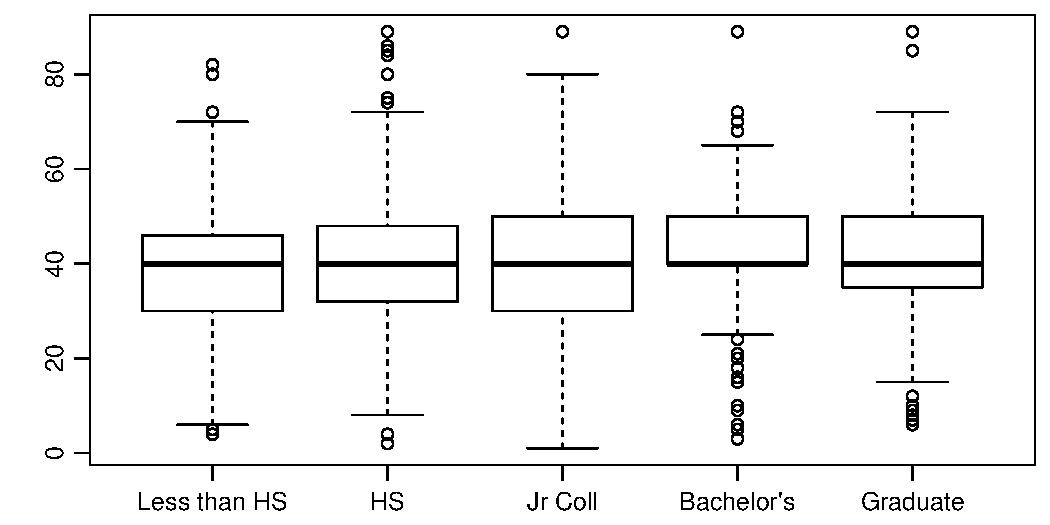
\includegraphics[width=\textwidth]{5-2_diff_two_mean/figures/hrs_edu/hrs_degree_box}
\end{center}

\end{frame}

%%%%%%%%%%%%%%%%%%%%%%%%%%%%%%%%%%%%

\begin{frame}[fragile]
\frametitle{Collapsing levels into two}

\begin{itemize}

\item Say we are only interested the difference between the number of hours worked per week by college and non-college graduates.

\pause

\item Then we combine the levels of education into two:
\begin{itemize}
\item \texttt{hs or lower} $\leftarrow$ less than high school or high school
\item \texttt{coll or higher} $\leftarrow$ junior college, bachelor's, and graduate
\end{itemize}

\end{itemize}

\end{frame}
%%%%%%%%%%%%%%%%%%%%%%%%%%%%%%%%%%%%

\begin{frame}
\frametitle{Exploratory analysis - another look}

\begin{center}
\begin{tabular}{lccc}
\hline
  		& $\bar{x}$ 	& $s$	& $n$ \\
\hline
coll or higher	& 41.8		& 15.14	& 505 \\
hs or lower	& 39.4		& 15.12	& 667 \\
\hline
\end{tabular}
$\:$ \\
\vspace{0.5cm}
$\:$ \\
\includegraphics[width=0.7\textwidth]{5-2_diff_two_mean/figures/hrs_edu/hrs_edu_hist}
\end{center}

\end{frame}

%%%%%%%%%%%%%%%%%%%%%%%%%%%%%%%%%%%

\begin{frame}
\frametitle{Parameter and point estimate}

\dq{We want to construct a 95\% confidence interval for the average difference between the number of hours worked per week by Americans with a college degree and those with a high school degree or lower. What are the parameter of interest and the point estimate?}

\pause

\begin{itemize}

\item \hl{Parameter of interest:} Average difference between the number of hours worked per week by \red{all}  Americans with a college degree and those with a high school degree or lower.
\[ \mu_{coll} - \mu_{hs} \]

\pause

\item \hl{Point estimate:} Average difference between the number of hours worked per week by \red{sampled}  Americans with a college degree and those with a high school degree or lower.
\[ \bar{x}_{coll} - \bar{x}_{hs} \]

\end{itemize}

\end{frame}

%%%%%%%%%%%%%%%%%%%%%%%%%%%%%%%%%%%

\begin{frame}[shrink]
\frametitle{Checking assumptions \& conditions}

\begin{enumerate}

\item \hl{Independence within groups: }
\begin{itemize}
\item Both the college graduates and those with HS degree or lower are sampled randomly.
\pause
\item 505 $<$ 10\% of all college graduates and 667 $<$ 10\% of all students with a high school degree or lower.
\end{itemize}
\pause
We can assume that the number of hours worked per week by one college graduate in the sample is independent of another, and the number of hours worked per week by someone with a HS degree or lower in the sample is independent of another as well.

\pause

\item \hl{Independence between groups: } \red{$\leftarrow$ new!} \\
Since the sample is random, the college graduates in the sample are independent of those with a HS degree or lower.

\pause

\item \hl{Sample size / skew:} \\
Both distributions look reasonably symmetric, and the sample sizes are at least 30, therefore we can assume that the sampling distribution of number of hours worked per week by college graduates and those with HS degree or lower are nearly normal. Hence the sampling distribution of the average difference will be nearly normal as well.

\end{enumerate}

\end{frame}

%%%%%%%%%%%%%%%%%%%%%%%%%%%%%%%%%%%

\begin{frame}
\frametitle{Confidence interval for difference between two means}

\begin{itemize}

\item All confidence intervals have the same form:
\[ \textcolor{orange}{point~estimate \pm ME} \]

\pause

\item And all $ \textcolor{orange}{ME = critical~value \times SE~of~point~estimate}$

\pause

\item In this case the point estimate is $\bar{x}_1 - \bar{x}_2$

\pause

\item Since the sample sizes are large enough, the critical value is $z^\star$

\pause

\item So the only new concept is the standard error of the difference between two means...

\end{itemize}

\pause

\formula{Standard error of the difference between two sample means}
{
\[ SE_{(\bar{x}_1 - \bar{x}_2)} = \sqrt{ \frac{s_1^2}{n_1} + \frac{s_2^2}{n_2} } \]
}

\end{frame}

%%%%%%%%%%%%%%%%%%%%%%%%%%%%%%%%%%%

\begin{frame}
\frametitle{Let's put things in context}

\dq{Calculate the standard error of the average difference between the number of hours worked per week by college graduates and those with a HS degree or lower.}

\twocol{0.5}{0.5}
{
\begin{tabular}{lccc}
\hline
			& $\bar{x}$ 	& $s$	& $n$ \\
\hline
coll or higher	& 41.8		& 15.14	& 505 \\
hs or lower	& 39.4		& 15.12	& 667 \\
\hline
\end{tabular}
}
{
\pause
\begin{eqnarray*}
SE_{(\bar{x}_{coll} - \bar{x}_{hs})} &=& \sqrt{ \frac{s_{coll}^2}{n_{coll}} + \frac{s_{hs}^2}{n_{hs}} } \\
\pause
&=& \sqrt{ \frac{15.14^2}{505} + \frac{15.12^2}{667} } \\
\pause
&=& 0.89
\end{eqnarray*}
}

\end{frame}

%%%%%%%%%%%%%%%%%%%%%%%%%%%%%%%%%%%

\begin{frame}
\frametitle{Confidence interval for the difference (cont.)}

\dq{Estimate (using a 95\% confidence interval) the average difference between the number of hours worked per week by Americans with a college degree and those with a high school degree or lower. 
\[ \bar{x}_{coll} = 41.8 \qquad \bar{x}_{hs} = 39.4 \qquad SE_{(\bar{x}_{coll} - \bar{x}_{hs})} = 0.89 \]}

\pause

\begin{eqnarray*}
(\bar{x}_{coll} - \bar{x}_{hs}) \pm z^\star \times SE_{(\bar{x}_{coll} - \bar{x}_{hs})} &=& (41.8 - 39.4) \pm 1.96 \times 0.89 \\
\pause
&=& 2.4 \pm 1.74 \\
\pause
&=& (0.66, 4.14)
\end{eqnarray*}


\end{frame}

%%%%%%%%%%%%%%%%%%%%%%%%%%%%%%%%%%%

\begin{frame}
\frametitle{Interpretation of a confidence interval for the difference}

\pq{Which of the following is the \underline{best} interpretation of the confidence interval we just calculated?}

\begin{enumerate}[(a)]
\item The difference between the average number of hours worked per week by college grads and those with a HS degree or lower is between 0.66 and 4.14 hours.
\solnMult{College grads work on average of 0.66 to 4.14 hours more per week than those with a HS degree or lower.}
\item College grads work on average 0.66 hours less to 4.14 hours more per week than those with a HS degree or lower.
\item College grads work on average 0.66 to 4.14 hours less per week than those with a HS degree or lower.
\end{enumerate}

\end{frame}

%%%%%%%%%%%%%%%%%%%%%%%%%%%%%%%%%%%

\begin{frame}
\frametitle{Reality check}

\dq{Do these results sound reasonable? Why or why not?}

\end{frame}


%%%%%%%%%%%%%%%%%%%%%%%%%%%%%%%%%%%

\subsection{Hypothesis tests for differences of means}

%%%%%%%%%%%%%%%%%%%%%%%%%%%%%%%%%%%

\begin{frame}
\frametitle{Setting the hypotheses}

\dq{What are the hypotheses for testing if there is a difference between the average number of hours worked per week by college graduates and those with a HS degree or lower?}

\pause

\begin{itemize}
\item[$H_0$:] $\mu_{coll} = \mu_{hs}$  \\
{\small There is no difference in the average number of hours worked per week by college graduates and those with a HS degree or lower. Any observed difference between the sample means is due to natural sampling variation (chance).}
\pause
\item[$H_A$:] $\mu_{coll} \neq \mu_{hs}$  \\
{\small There is a difference in the average number of hours worked per week by college graduates and those with a HS degree or lower.}
\end{itemize}

\end{frame}

%%%%%%%%%%%%%%%%%%%%%%%%%%%%%%%%%%%

\begin{frame}[shrink]
\frametitle{Calculating the test-statistic and the p-value}

\begin{itemize}
\item[$H_0$:] $\mu_{coll} = \mu_{hs} \rightarrow$ \red{$\mu_{coll} - \mu_{hs} = 0$} \\
\item[$H_A$:] $\mu_{coll} \neq \mu_{hs} \rightarrow \mu_{coll} - \mu_{hs} \ne 0$  \\
\item[]
\item[] $\bar{x}_{coll} - \bar{x}_{hs} = 2.4$, $SE_(\bar{x}_{coll} - \bar{x}_{hs}) = 0.89$
\end{itemize}


\pause

\twocol{0.5}{0.5}
{
\begin{center}
\includegraphics[width=\textwidth]{5-2_diff_two_mean/figures/hrs_edu/hrs_norm}
\end{center}
}
{
\pause
\small{
\begin{eqnarray*}
Z &=& \frac{(\bar{x}_{coll} - \bar{x}_{hs}) - 0}{ SE_{(\bar{x}_{coll} - \bar{x}_{hs})} } \\
\pause
&=& \frac{2.4}{0.89} = 2.70 \\
\pause
upper~tail &=&  1 -  0.9965 = 0.0035 \\
\pause
p-value &=& 2 \times 0.0035 = 0.007
\end{eqnarray*}
}
}

\end{frame}

%%%%%%%%%%%%%%%%%%%%%%%%%%%%%%%%%%%

\begin{frame}
\frametitle{Conclusion of the test}

\pq{Which of the following is correct based on the results of the hypothesis test we just conducted?}

{\small
\begin{enumerate}[(a)]
\item There is a 0.7\% chance that there is no difference between the average number of hours worked per week by college graduates and those with a HS degree or lower.
\solnMult{Since the p-value is low, we reject $H_0$. The data provide convincing evidence of a difference between the average number of hours worked per week by college graduates and those with a HS degree or lower.}
\item Since we rejected $H_0$, we may have made a Type 2 error.
\item Since the p-value is low, we fail to reject $H_0$. The data do not provide convincing evidence of a difference between the average number of hours worked per week by college graduates and those with a HS degree or lower.
\end{enumerate}
}

\end{frame}

%%%%%%%%%%%%%%%%%%%%%%%%%%%%%%%%%%%%